\documentclass{beamer}

\usepackage{graphicx}
\usepackage{bibentry}
\graphicspath{ {./images/} }

\title{Analyse von Pflanzenwachstum auf Basis von 3D-Punktwolken}
%\subtitle{Vergleich zweier Frameworks in einem verteilten System zum lösen linearer Gleichungsysteme.}

\author{Jakob Görner} 
\institute[Computer Vision] 
{HSNR - Master Arbeit - Vortrag \\ % Your institution for the title page
\medskip
\textit{jakob.goerner@stud.hn.de} % Your email address

}

%\usetheme{lucid}
\begin{document}
	\frame {
		\titlepage
	}
	\frame {
		\frametitle{Inhalt} 
		\tableofcontents
	}
\section{Ziele}
	\frame {
		\frametitle{Ziele} 
		\begin{itemize}
			\item Analyse von Pflanzen mittels 3D-Punktwolken
			\item Generierung von Punktwolken auf Basis von Bildern
			\item Kernprobleme
			\begin{itemize}
				\item Entfernung des Hintergrundes
				\item Segmentierung der Pflanze
				\item Skalierung der Punktwolken ist unbekannt.
			\end{itemize}
			\item REST-Interface zum einspielen von Datensätzen und ansteuern der Funktionalitäten.
			\item Datenübertragung zum Server sollte gering gehalten werden.
		\end{itemize}
	}
\section{Punktwolken Generieren}
	\frame {
		\frametitle{Generierung von Punktwolken auf Basis von Bildern} 
		\begin{itemize}
				\item Einsatz von spezieller Hardware sollte nicht nötig sein.
				\item Da es viele bestehende Lösungen für das Problem existieren wird auf eine existierende Implementationen zurück gegriffen.
				\item Voraussetzungen an die Implementation
			\begin{itemize}
				\item Keine Information über Kamera Position und Ausrichtung
				\item Gegebenenfalls keine Information über die Reihenfolge der Bilder
			\end{itemize}
			\item Evaluation mehrerer Implementationen
			\begin{itemize}
				\item Open Drone Map \cite{ODM}
				\item Colmap \cite{schoenberger2016sfm}
				\item AliceVision (Meshroom) \cite{Moulon2012}
				\item OpenMVG \cite{moulon2016openmvg} 
				\item OpenCV SFM Pipeline
			\end{itemize}
			\item Open Drone Map und Colmap liefern gute Ergebnisse
			\item Open Drone Map(ODM) wesentlich performanter als Colmap (schnellere Berechnung bei weniger Ressourcen-Verbrauch)
			\item ODM liefert gute Schätzung der Normalen.
		\end{itemize}
		
	}
	\frame {
		\frametitle{Generierung von Punktwolken auf Basis von Bildern} 
		
		\begin{columns}[T] % align columns
			\begin{column}{.48\textwidth}
			\begin{figure}[h!]
  				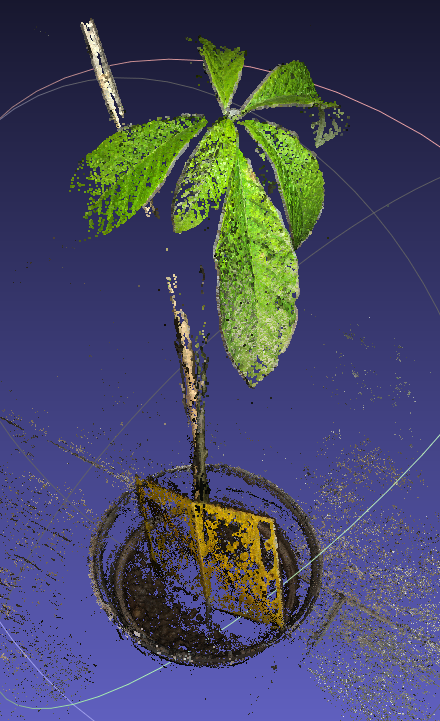
\includegraphics[width=5cm,height=6cm,keepaspectratio]{ColmapPointCloudAvocado5}
  				\caption{Colmap Punktwolke - 30 Bilder}
  				\label{ColmapPointCloudAvocado5}
			\end{figure}
			\end{column}%
		\hfill%
			\begin{column}{.48\textwidth}
			
			\begin{figure}[h!]
  				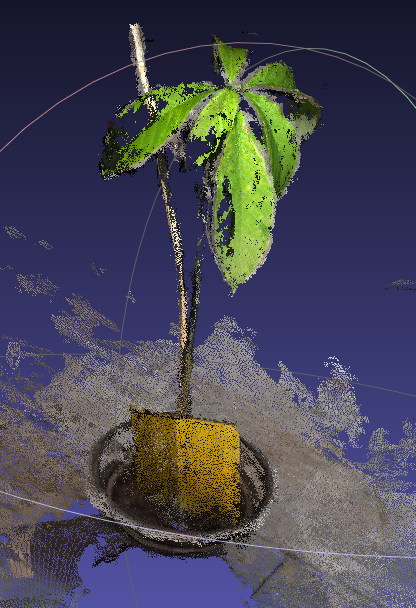
\includegraphics[width=5cm,height=6cm,keepaspectratio]{ODMPointCloudAvocado5}
  				\caption{ODM Punktwolke - 30 Bilder}
  				\label{ODMPointCloudAvocado5}
			\end{figure}
			\end{column}%
		\end{columns}
	}
\section{Registration Pipeline}
	\frame {
		\frametitle{Registration} 
		\begin{columns}[T] % align columns
			\begin{column}{.58\textwidth}
				\begin{itemize}
					\item Punktwolken aneinander ausrichten
					\item Abstand zwischen einzelnen Punkten minimieren
					\item Wird in der Regel dazu benutzt um mehrere Punktwolken zu einer gesamtheitlichen Szene zu verbinden.
					\item Initiale Angleichung mittels SIFT 3D \cite{Sift3D}
					\item Finale Angleichung via Iterative Closest Point Algorithmus (ICP) \cite{ICP}
					\item Problem: Skalierung der Punktwolken ist nicht bekannt.
				\end{itemize}
			\end{column}%
		\hfill%
			\begin{column}{.38\textwidth}
			
			\begin{figure}[h!]
  				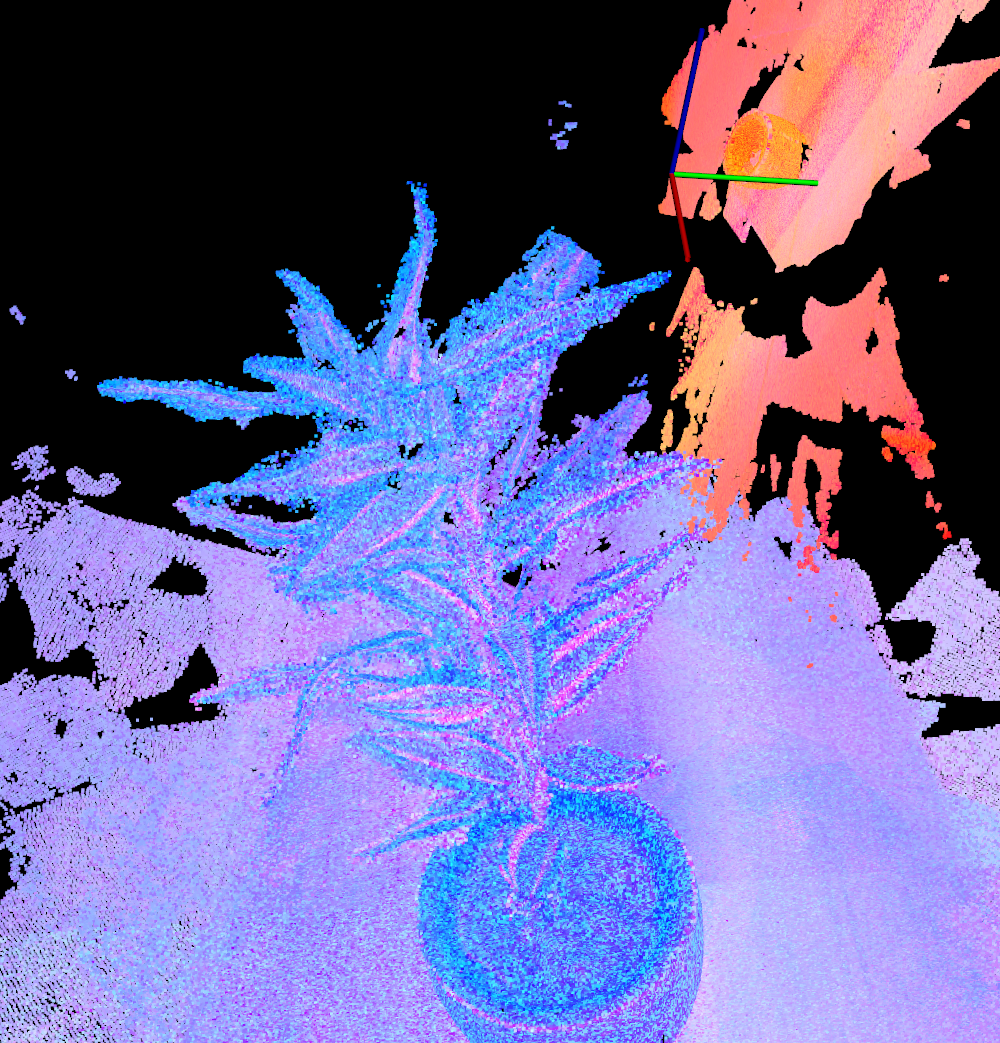
\includegraphics[scale=0.125]{UnalignedClouds}
  				\caption{Ausgangsposition zweier Punktwolken}
  				\label{UnalignedClouds}
			\end{figure}
			\end{column}%
		\end{columns}
		
	}
	\frame {
		\frametitle{Registration}
		
		\begin{columns}[T] % align columns
			\begin{column}{.48\textwidth}
			\begin{figure}[h!]
  				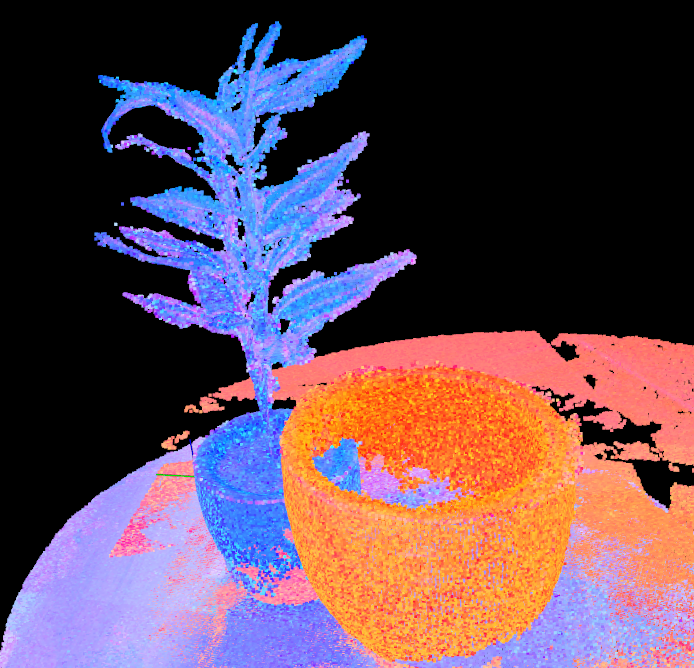
\includegraphics[width=5cm,height=7cm,keepaspectratio]{SIFTAlignment}
  				\caption{SIFT Alignment}
  				\label{SIFTAlignment}
			\end{figure}
			\end{column}%
		\hfill%
			\begin{column}{.48\textwidth}
			
			\begin{figure}[h!]
  				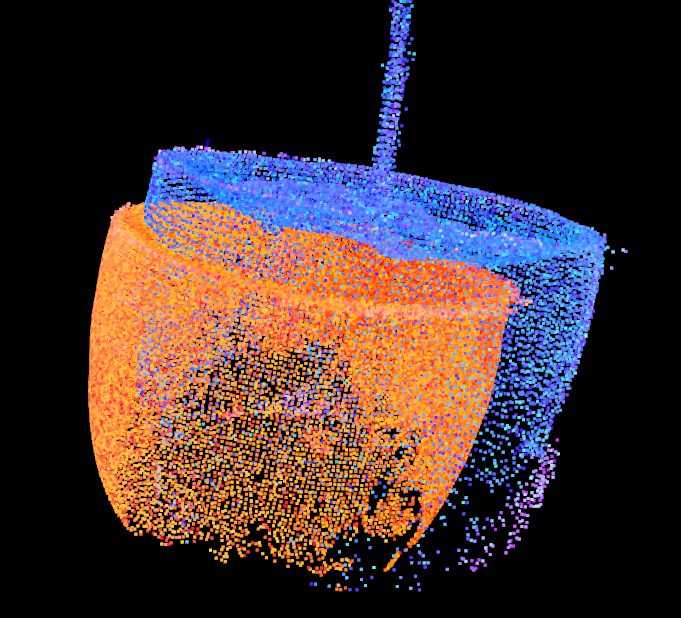
\includegraphics[width=5cm,height=7cm,keepaspectratio]{FinalAlignment}
  				\caption{ICP Alignment}
  				\label{FinalAlignment}
			\end{figure}
			\end{column}%
		\end{columns}
	}
	\frame {
		\frametitle{Background Removel Pipeline} 
		\begin{itemize}
			\item Vorraussetzungen: Vor dem pflanzen muss ein Datensatz von Bildern aufgenommen werden und eine Punktwolke generiert werden
			\item Registrierung der Hintergrund-Punktwolke $b$ mit Punktwolke zum Zeitpunkt $t_i$
			\item Entferne Punkte von $t_i$ die nahe Punkten aus $b$ sind. 
			\item Wichtig: $b$ darf seine Skalierung nicht ändern.
			\item Vor und Nachbearbeitung der Punkwolken ist nötig.
 		\end{itemize}
	}
	\frame {
		\frametitle{Wachstums-Analyse Pipeline} 
		\begin{columns}[T] % align columns
			\begin{column}{.48\textwidth}
			\begin{itemize}
				\item Registrierung zweier Punktwolken zu verschiedenen Zeitpunkten
				\item Schätzung des Wachstums auf Basis der Ausdehnung der Punktwolke.
				\item Es kann das Volumen geschätzt werden.
				\item Es kann die Höhe geschätzt werden.
			\end{itemize}
			\end{column}%
		\hfill%
			\begin{column}{.48\textwidth}
			\begin{figure}[h!]
  				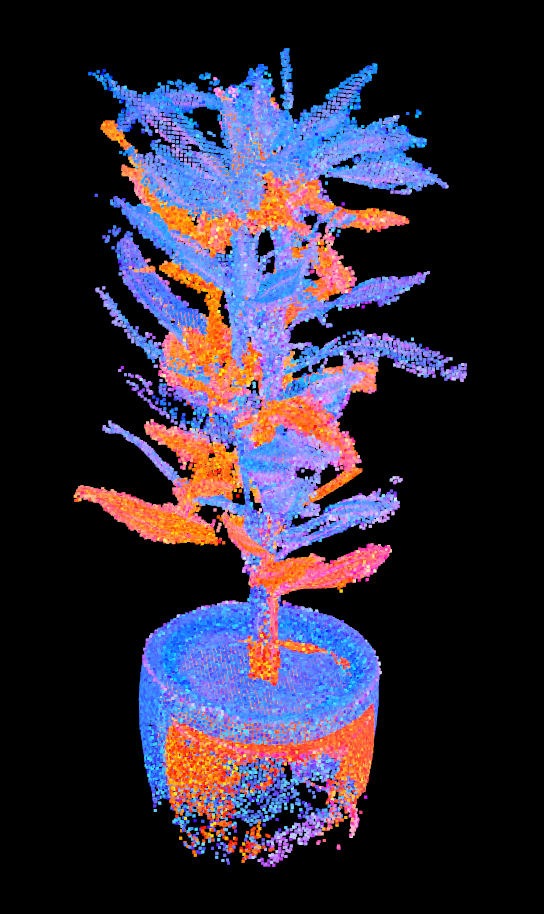
\includegraphics[scale=0.2]{MatchedTimestamps}
  				\caption{Registrierung zweier Zeitpunkte}
  				\label{MatchedTimestamps}
			\end{figure}
			\end{column}%
		\end{columns}
		
	}
\section{Binary Classifier}
	\frame {
		\frametitle{Klassifizierung von Blättern und Stielen}
		
		\begin{columns}[T] % align columns
			\begin{column}{.58\textwidth}
				\begin{itemize}
					\item Ansatz über Hauptkrümmung der Punkte \cite{ThreeBasics}.
					\item Bilde Maß aus Werten der Hauptkrümmung für ein Schwellwertverfahren.
					\item Die Hauptkrümmung eines Punktes $p_i$ wird über benachbarte Punkte $N_i$ berechnet.
					\item Es wird die Kovarianz-Matrix $C_i$ zwischen $p_i$ und den Punkten in $N_i$ gebildet. 
					\item Aus den Eigenwerten von $C_i$ können die beiden Werte der Hauptkrümmung gebildet werden.
				\end{itemize}
			\end{column}%
		\hfill%
			\begin{column}{.38\textwidth}
			\begin{figure}[h!]
  				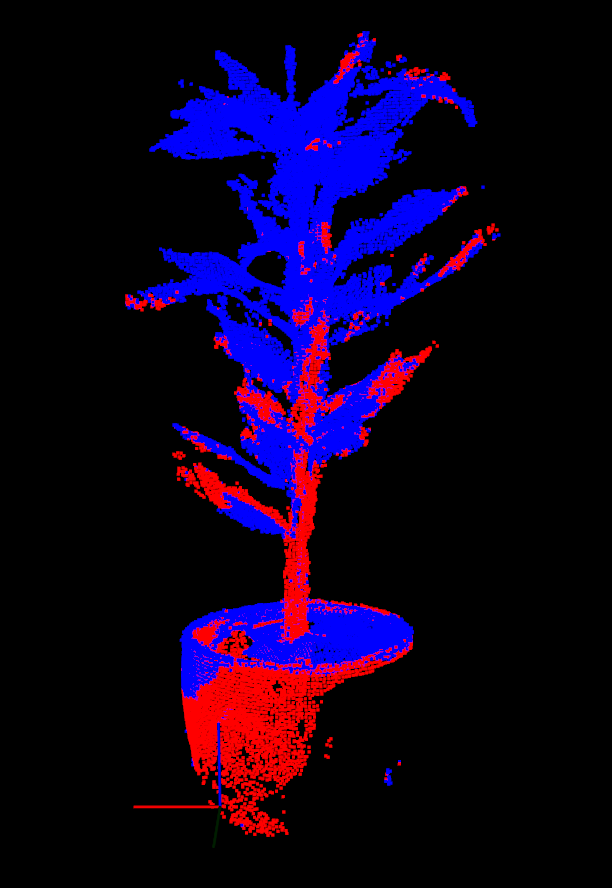
\includegraphics[scale=0.2]{ClassifiedPointCloud}
  				\caption{Punktwolke nach Klassifikation. Rot: Stamm Blau: Blatt}
  				\label{ClassifiedPointCloud}
			\end{figure}
			\end{column}%
		\end{columns}
	}
	\frame {
		\frametitle{Analyse der Blätter}
		\begin{itemize}
			\item Punkte die als Stiel klassifiziert wurden werden aus der Punktwolke entfernt.
			\item Zählen der Blätter mittels Region Growing \cite{RegionGrowing}.
			\item Analyse des Blätterwachstums über Zeit.
			\item Blättern die sich berühren werden zusammen gezählt.
			\item Mögliche Lösung ist ein Filter der überlappende Punkte und Ränder erkennt und entfernt.
			\item weitere Möglichkeit über Analyse von Kanten. 
			\begin{itemize}
				\item Blätter haben in der Regel konvexe Formen.
				\item Es gibt ausnahmen die aus zusammenhängenden konvexen Formen bestehen.
			\end{itemize}	 
		\end{itemize}
	}
	\frame {
		\frametitle{Analyse der Stielen}

		\begin{columns}[T] % align columns
			\begin{column}{.48\textwidth}
				\begin{itemize}
					\item Entferne alle Punkte die als Blätter klassifiziert wurden.
					\item Punktwolke der Stiele skelettieren.
					\item Erkannte Stiele können in einer Baumstruktur abgelegt werden.
					\item Baumstruktur ermöglicht das Zählen von Stielen über Zeit.
				\end{itemize}
			\end{column}%
		\hfill%
			\begin{column}{.48\textwidth}
				\begin{figure}[h!]
					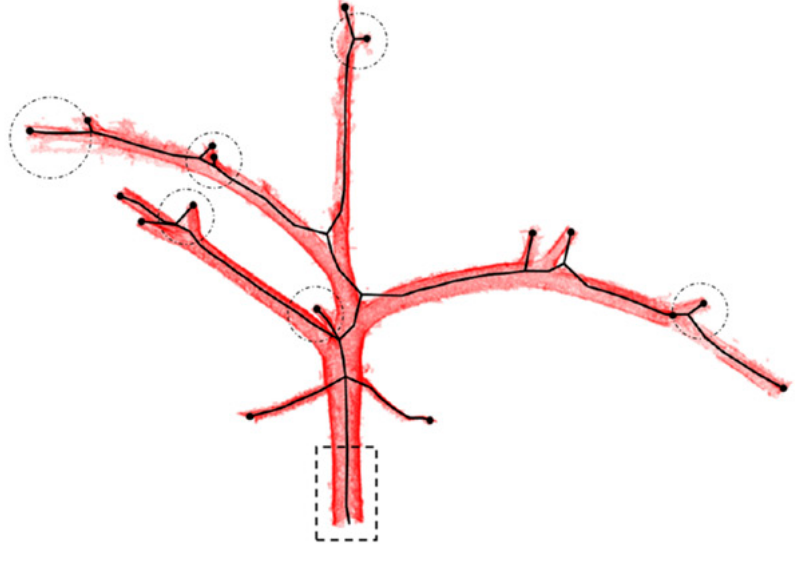
\includegraphics[scale=0.2]{StemSkelet}
					\caption{Skelettierung der Triebe \cite{ThreeBasics}}
					\label{StemSkelet}
			  	\end{figure}
			\end{column}%
		\end{columns}
	}
	\frame {
		\frametitle{Schnittstelle}

		\begin{itemize}
			\item Datensatz erstellen (Bildern des Hintergrunds hinzufügen).
			\item Messpunkt hinzufügen.
			\begin{itemize}
				\item Datensatz mit Bildern von aktuellem Wachstum zum Messpunkt $t$ hinzufügen.
				\item Pipelines werden gestartet. 
			\end{itemize}
			\item Liste der bereits berechneten Messpunkt zu einem Datensatz.
			\item Details zu Messpunkt $t$.
			\begin{itemize}
				\item Wachstum seit vorherigem Messpunkt.
				\item Anzahl der Blätter.
				\item Anzahl der Stielen.
				\item Volumen der Pflanze.
			\end{itemize}
		\end{itemize}
	}
	\begin{frame}[allowframebreaks]
        \frametitle{Referenzen}
        \bibliographystyle{ieeetr}
        \bibliography{./bibleografie.bib}
\end{frame}

% \[\frac{-b \pm \sqrt{b^2 - c}}{2a}\]

\end{document}
